\documentclass{sigchi}

% Use this section to set the ACM copyright statement (e.g. for
% preprints).  Consult the conference website for the camera-ready
% copyright statement.

% Copyright
\CopyrightYear{2016}
%\setcopyright{acmcopyright}
\setcopyright{acmlicensed}
%\setcopyright{rightsretained}
%\setcopyright{usgov}
%\setcopyright{usgovmixed}
%\setcopyright{cagov}
%\setcopyright{cagovmixed}
% DOI
\doi{http://dx.doi.org/10.475/123_4}
% ISBN
\isbn{123-4567-24-567/08/06}
%Conference
\conferenceinfo{CHI'16,}{May 07--12, 2016, San Jose, CA, USA}
%Price
\acmPrice{\$15.00}

% Use this command to override the default ACM copyright statement
% (e.g. for preprints).  Consult the conference website for the
% camera-ready copyright statement.

%% HOW TO OVERRIDE THE DEFAULT COPYRIGHT STRIP --
%% Please note you need to make sure the copy for your specific
%% license is used here!
 \toappear{
 Permission to make digital or hard copies of all or part of this work
 for personal or classroom use is granted without fee provided that
 copies are not made or distributed for profit or commercial advantage
 and that copies bear this notice and the full citation on the first
 page. Copyrights for components of this work owned by others than ACM
 must be honored. Abstracting with credit is permitted. To copy
 otherwise, or republish, to post on servers or to redistribute to
 lists, requires prior specific permission and/or a fee. Request
 permissions from \href{mailto:Permissions@acm.org}{Permissions@acm.org}. \\
 \emph{CHI '16},  May 07--12, 2016, San Jose, CA, USA \\
 ACM xxx-x-xxxx-xxxx-x/xx/xx\ldots \$15.00 \\
 DOI: \url{http://dx.doi.org/xx.xxxx/xxxxxxx.xxxxxxx}
 }

% Arabic page numbers for submission.  Remove this line to eliminate
% page numbers for the camera ready copy
% \pagenumbering{arabic}

% Load basic packages
\usepackage[brazil]{babel}
\usepackage[utf8]{inputenc}
\usepackage{balance}       % to better equalize the last page
\usepackage{graphics}      % for EPS, load graphicx instead 
\usepackage[T1]{fontenc}   % for umlauts and other diaeresis
\usepackage{txfonts}
\usepackage{mathptmx}
\usepackage[pdflang={pt-BR},pdftex]{hyperref}
\usepackage{color}
\usepackage{booktabs}
\usepackage{textcomp}

% Some optional stuff you might like/need.
\usepackage{microtype}        % Improved Tracking and Kerning
% \usepackage[all]{hypcap}    % Fixes bug in hyperref caption linking
\usepackage{ccicons}          % Cite your images correctly!
% \usepackage[utf8]{inputenc} % for a UTF8 editor only

% If you want to use todo notes, marginpars etc. during creation of
% your draft document, you have to enable the "chi_draft" option for
% the document class. To do this, change the very first line to:
% "\documentclass[chi_draft]{sigchi}". You can then place todo notes
% by using the "\todo{...}"  command. Make sure to disable the draft
% option again before submitting your final document.
\usepackage{todonotes}

% Paper metadata (use plain text, for PDF inclusion and later
% re-using, if desired).  Use \emtpyauthor when submitting for review
% so you remain anonymous.
\def\plaintitle{Melhorando a qualidade de decisões colaborativas para uma cidade inteligente}
\def\plainauthor{Carlos Elmadjian, Tarcisio Pereira}
\def\emptyauthor{}
\def\plainkeywords{escrever; aqui; obrigatório}
\def\plaingeneralterms{Documentation, Standardization}

% llt: Define a global style for URLs, rather that the default one
\makeatletter
\def\url@leostyle{%
  \@ifundefined{selectfont}{
    \def\UrlFont{\sf}
  }{
    \def\UrlFont{\small\bf\ttfamily}
  }}
\makeatother
\urlstyle{leo}

% To make various LaTeX processors do the right thing with page size.
\def\pprw{8.5in}
\def\pprh{11in}
\special{papersize=\pprw,\pprh}
\setlength{\paperwidth}{\pprw}
\setlength{\paperheight}{\pprh}
\setlength{\pdfpagewidth}{\pprw}
\setlength{\pdfpageheight}{\pprh}

% Make sure hyperref comes last of your loaded packages, to give it a
% fighting chance of not being over-written, since its job is to
% redefine many LaTeX commands.
\definecolor{linkColor}{RGB}{6,125,233}
\hypersetup{%
  pdftitle={\plaintitle},
% Use \plainauthor for final version.
%  pdfauthor={\plainauthor},
  pdfauthor={\emptyauthor},
  pdfkeywords={\plainkeywords},
  pdfdisplaydoctitle=true, % For Accessibility
  bookmarksnumbered,
  pdfstartview={FitH},
  colorlinks,
  citecolor=black,
  filecolor=black,
  linkcolor=black,
  urlcolor=linkColor,
  breaklinks=true,
  hypertexnames=false
}

% create a shortcut to typeset table headings
% \newcommand\tabhead[1]{\small\textbf{#1}}

% End of preamble. Here it comes the document.
\begin{document}

\title{\plaintitle}

\numberofauthors{2}
\author{%
  \alignauthor{Carlos Elmadjian\\
    \affaddr{IME / USP}\\
    \affaddr{São Paulo, Brasil}\\
    \email{elmad@ime.usp.br}}\\
  \alignauthor{Tarcisio Pereira\\
    \affaddr{IME / USP}\\
    \affaddr{São Paulo, Brasil}\\
    \email{tarcisio1@hotmail.com}}\\
}

\maketitle

\begin{abstract}
  resumo em 150 palavras.
\end{abstract}

\category{H.5.m.}{Information Interfaces and Presentation
  (e.g. HCI)}{Miscellaneous} \category{See
  \url{http://acm.org/about/class/1998/} for the full list of ACM
  classifiers. This section is required.}{}{}

\keywords{\plainkeywords}

\section{Introdução}
- introdução explicando a ideia do trabalho (e o título)\\
- descrição de trabalhos correlatos\\
- motivação e justificativas para o trabalho (referências resumidas na disciplina AQUI)\\


\begin{figure}
\centering
  
\includegraphics[width=0.9\columnwidth]{figures/sigchi-logo}
  \caption{Insert a caption below each figure. Do not alter the
    Caption style.  One-line captions should be centered; multi-line
    should be justified. }~\label{fig:figure1}
\end{figure}


\begin{table}
  \centering
  \begin{tabular}{l r r r}
    % \toprule
    & & \multicolumn{2}{c}{\small{\textbf{Test Conditions}}} \\
    \cmidrule(r){3-4}
    {\small\textit{Name}}
    & {\small \textit{First}}
      & {\small \textit{Second}}
    & {\small \textit{Final}} \\
    \midrule
    Marsden & 223.0 & 44 & 432,321 \\
    Nass & 22.2 & 16 & 234,333 \\
    Borriello & 22.9 & 11 & 93,123 \\
    Karat & 34.9 & 2200 & 103,322 \\
    % \bottomrule
  \end{tabular}
  \caption{Table captions should be placed below the table. We
    recommend table lines be 1 point, 25\% black. Minimize use of
    table grid lines.}~\label{tab:table1}
\end{table}


\section{Ferramenta E-Voz}
- descrição do protótipo\\
- imagens com telas dos protótipos\\
- propósito do protótipo\\
- diferença para outras aplicações (estado da arte)\\



\begin{figure*}
  \centering
  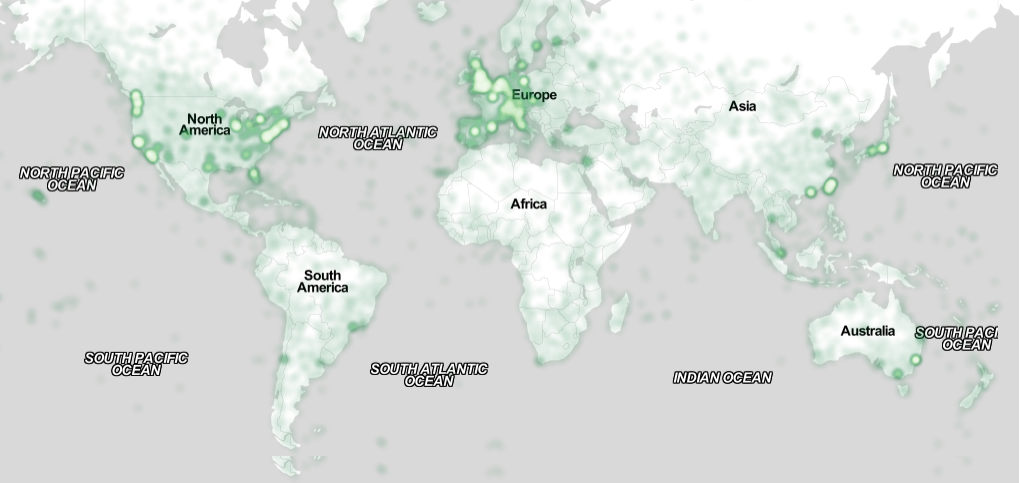
\includegraphics[width=1.75\columnwidth]{figures/map}
  \caption{In this image, the map maximizes use of space. You can make
    figures as wide as you need, up to a maximum of the full width of
    both columns. Note that \LaTeX\ tends to render large figures on a
    dedicated page. Image: \ccbynd~ayman on
    Flickr.}~\label{fig:figure2}
\end{figure*}


\section{Protocolo experimental}
- planejamento das atividades\\
- como as pessoas foram abordadas\\
- locais de realização do experimento\\
- descrição dos procedimentos, incluindo imagens das telas mostrando os procedimentos\\
- justificativa dos procedimentos\\


\section{Resultados}
- perfil dos participantes (idade, residência, sexo)\\
- estatísticas das respostas\\
- análise estatística\\
- tabelas com resultados\\


\section{Discussão}
Os dados reforçam a hipótese do viés de disponibilidade~\cite{tversky:1973} na tomada de decisão dos participantes. No grupo que interagiu primeiro com o protótipo I e depois com o II, nota-se uma alteração no critério de escolha da prioridade dos problema com o aumento de informações que subsidiam a tarefa. O mesmo não se observa no grupo que inicia a interação pelo protótipo II e depois segue para o I. Quando questionados sobre a mudança de postura, a maior parte dos participantes reconheceu utilizar um critério individualista quando não havia informações estatísticas disponíveis sobre a cidade, o que parece indicar que o recurso impacta positivamente para tomada de decisões mais altruístas ou coletivistas.

\section{Limitações e trabalho futuro}
- quantidade de participantes\\
- avaliação de outros fatures que contribuem para a interação colaborativa (rede social, por exemplo)

\section{Conclusão}
- oferecer recursos para melhora de decisão em plataformas colaborativas sem onerar a usabilidade de interfaces pode inicialmente ser um desafio, mas os efeitos aparentes tanto na qualidade da interação (percepção dos usuários) quanto na utilidade e resultados indicam um benefício significativo.


\section{Agradecimentos}

Agradecemos a todos os participantes que se submeteram voluntariamente ao experimento e aos nossos revisores, com seus comentários e críticas valiosas para o trabalho.


\balance{}


% BALANCE COLUMNS
\balance{}

% REFERENCES FORMAT
% References must be the same font size as other body text.
\bibliographystyle{SIGCHI-Reference-Format}
\bibliography{sample}

\end{document}

%%% Local Variables:
%%% mode: latex
%%% TeX-master: t
%%% End:
